
\section{Week 10: Reproducible ML Workflow Studio}
\textbf{Monday, 9 November 2026, 14:00--17:00.} The class contains 60 minutes of explanation and 120 minutes of practice. H1 uses 45/15 minutes, H2 uses 15/45, and H3 is a 60-minute studio. Eight core exercises and two optional challenges are formative in-class practice, not new weekly graded homework. The next scheduled meeting is the written and oral midterm examination; this studio does not replace either examination.

The goal is a portable handover: another interpreter receives frozen files, checks their contract, reconstructs a declared model, and compares predictions by stable row identity. A matching screenshot, aggregate score or second notebook variable is not sufficient. Week 9 studied where a model fails; Week 10 asks whether the evidence supporting that analysis can travel.

\subsection{Computational replay has a bounded meaning}
Here, replay means recomputing predictions from the same frozen input records and declared procedure. A new interpreter and working directory remove the notebook's global variables and fitted-object memory. They do not create a new dataset, machine, package environment or physical experiment. Thus numerical agreement is narrower than independent scientific replication. A reproducible model can still be inaccurate or inapplicable.

A two-row counterexample clarifies the distinction between score and prediction identity. Errors $[0,2]$ and $[2,0]$ both have MAE 1, but fail on different observations. Compare aligned prediction vectors, not only their mean loss.

\section{Stable identity, not a seed alone}
A seeded permutation selects positions in an ordered array. If the array order changes first, the same positions may identify different observations. Assign source IDs before shuffling and persist them with their measured values. To reconstruct a cohort, build an ID-keyed lookup and iterate over the saved ID sequence. A set comparison verifies membership; a sequence comparison additionally verifies alignment.

The partition contract requires unique row IDs, no duplicates within any split, pairwise disjoint train/validation/test sets, the expected counts, and a union equal to the full frozen dataset. Disjointness alone does not catch omitted rows. Source row IDs are version-specific dataset identifiers, not globally stable patient identities or predictive features.

\section{The packaged regression fixture and its limits}
The original Week 10 material used scikit-learn's bundled diabetes regression dataset. We retain its 442 observations and 10 numeric inputs but call \texttt{load\_diabetes(scaled=False)}. The default loader returns globally centered/scaled inputs; raw loading makes the boundary of training-only fitted preprocessing explicit. We do not assign medical interpretations to individual features.

\textbf{Use boundary:} this is a statistical workflow exercise, not diagnosis, treatment guidance, causal discovery or external clinical validation. A random-row teaching split cannot establish future-time, new-site or clinical deployment validity. Dataset documentation also cautions that some feature meanings are not fully explicit.

One seeded permutation reserves 265 training, 88 validation and 89 final-test rows. Store exact floats, feature names, row IDs and split lists. The notebook checks finite numeric values, shape, counts and ID membership before fitting.

\subsection{An executable interface}
The CSV header must exactly match \texttt{row\_id}, the ten declared feature names in canonical order, and \texttt{target}. Duplicate IDs, non-finite values and reordered columns are rejected. Strict rejection is appropriate for a positional model interface; a separately declared and tested name adapter may create a valid canonical interface. Silently guessing feature order is not an acceptable repair.

These checks establish well-formedness relative to a contract, not scientific validity. A finite label can still be wrong, a unique ID can be attached to a wrong observation, and a correctly shaped dataset can be biased.

\section{Baseline, selection and held-out evidence}
Declare four candidates before final evaluation: a training-target median baseline and training-scaled Ridge models with $\alpha\in\{1,20,100\}$. A median minimizes $\sum_i|y_i-c|$ over constant predictions $c$. For an even sample size, any value between the two middle order statistics is a minimizer. That training property does not guarantee the best held-out score.

For the standardized design matrix $Z$, scikit-learn Ridge uses a residual-sum-of-squares objective plus an L2 penalty:
\[
 \min_{b,\beta}\ \sum_{i\in\mathrm{train}}(y_i-b-z_i^\mathsf T\beta)^2+\alpha\sum_j\beta_j^2.
\]
The intercept is not penalized in this formulation. Standardization and all coefficients are fitted on training data only. Stronger regularization changes the fitted function and coefficient norm; validation MAE need not improve monotonically. The training objective and selection metric need not be identical.

Choose the lowest validation MAE, breaking exact ties by the declared order: median, Ridge 1, Ridge 20, Ridge 100. Freeze the selected candidate before opening final-test results. The replay program refits this already selected candidate on training rows; it does not redo selection or refit on training plus validation.

\begin{figure}[htbp]\centering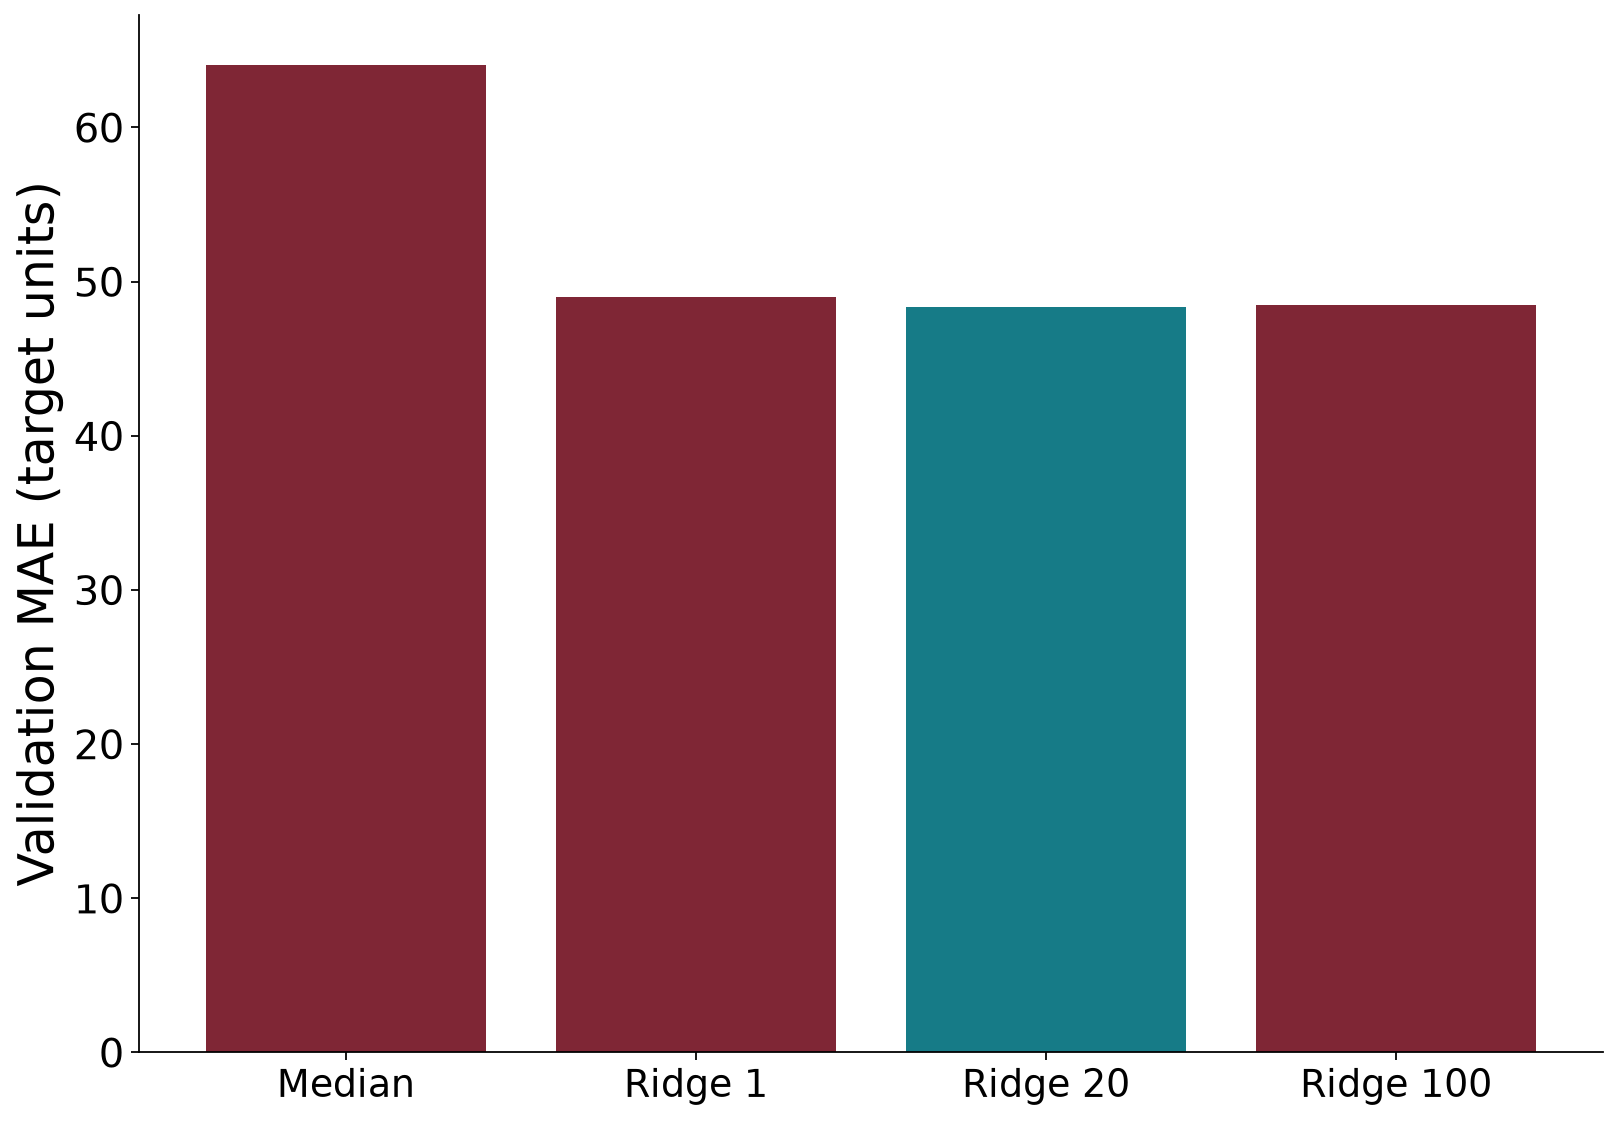
\includegraphics[width=.78\textwidth]{figures/week10/w10-validation-selection.png}\caption{Actual validation comparison on 88 rows. The reference run selects Ridge 20. Students retain their own actual environment and outputs.}\end{figure}

Report the selected candidate and the predeclared median baseline on the same 89 final-test observations. The residual convention is prediction minus observation; positive means overprediction. Inspect one actual large-residual source ID and its observed/predicted values. Do not infer a clinical mechanism from that row or tune alpha after inspecting it.

\begin{center}\begin{tabular}{lrrr}\toprule Candidate & Test n & MAE & RMSE\\\midrule
median & 89 & 65.280899 & 79.418957 \\
ridge-20 & 89 & 48.325756 & 59.411283 \\
\bottomrule\end{tabular}\end{center}

\begin{figure}[htbp]\centering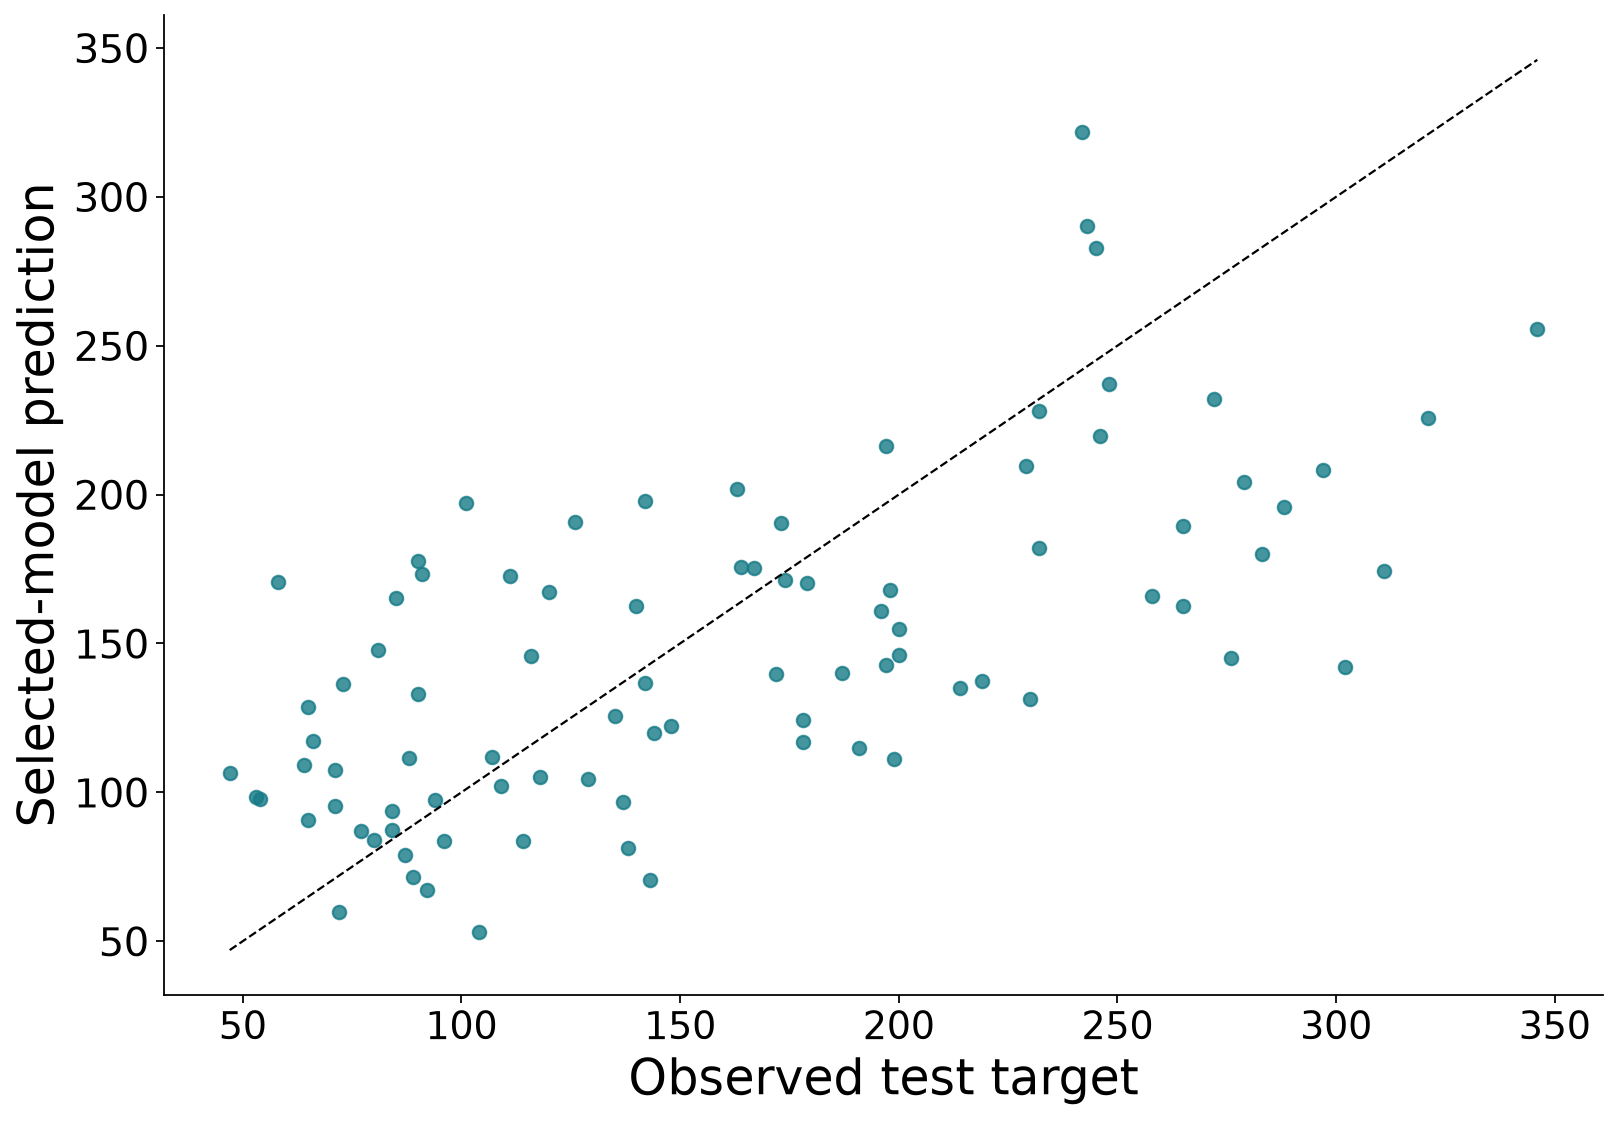
\includegraphics[width=.72\textwidth]{figures/week10/w10-test-parity.png}\caption{Actual selected-model final-test predictions. A later perfect computational replay does not remove these prediction errors against outcomes.}\end{figure}

\section{A checkable function explanation}
For $z_j=(x_j-\mu_j)/s_j$, standardized coefficient $\beta_j$ gives
\[
 \beta_j^{\mathrm{raw}}=\frac{\beta_j}{s_j},\qquad
 b^{\mathrm{raw}}=b-\sum_j\frac{\beta_j\mu_j}{s_j},\qquad
 f(x)=b^{\mathrm{raw}}+\sum_j\beta_j^{\mathrm{raw}}x_j.
\]
Reconstruct predictions and compare them to the pipeline. Increasing one input by $0.1s_j$ changes the fitted prediction by $0.1\beta_j$, with other coordinates fixed. This is an exact property of the additive fitted function, up to numerical tolerance. It need not correspond to a feasible causal or clinical intervention, especially with correlated features.

If the selected candidate were the constant median, this feature interpretation would not apply. The notebook then inspects the separately predeclared Ridge-20 candidate and records its name. Do not silently interpret a different candidate as the selected one.

\section{What belongs in the handover}
The payload has six required files:
\begin{center}\begin{tabular}{ll}\toprule File & Role\\\midrule
\texttt{frozen.csv} & Exact source IDs, features and target\\
\texttt{split.json} & Ordered training, validation and test IDs\\
\texttt{config.json} & Feature order, choices, selected candidate, versions\\
\texttt{replay.py} & Readable validation and fitting procedure\\
\texttt{reference-predictions.csv} & ID-aligned reference outcomes/predictions\\
\texttt{result.json} & Validation/test evidence and limitations\\\bottomrule\end{tabular}\end{center}
A separate \texttt{manifest.json} records the SHA-256 of each payload. It does not hash itself, which would be circular. The exported ZIP also retains actual plots, student responses and the current outer evidence record. The inner reference payload remains frozen.

\subsection{Integrity is not authentication}
SHA-256 detects changed bytes relative to a known reference digest. Parsing records checks a different identity. Appending a blank CSV line can preserve parsed rows while changing its hash. An unsigned manifest does not authenticate an unknown sender: someone able to replace both payload and digest can create another internally consistent package. Neither hashes nor schemas validate scientific labels or a performance claim.

The lab avoids loading a model pickle by reconstructing from CSV, JSON and readable source. Pickle-based loaders may execute arbitrary code. Executing Python source is also consequential: review and trust the generated runner before running it. A checksum does not make arbitrary downloaded code safe.

\section{Replay outside notebook memory}
The notebook launches a new Python interpreter in a new temporary working directory, passing only an explicit handover path and output path. The notebook copies the complete bundle into a new temporary directory and launches its reviewed runner with a separate interpreter. The runner verifies the required-file set and hashes, validates schema and split membership, reads the saved reference-prediction CSV and requires the exact test-ID sequence and observed targets. It then refits the frozen candidate and compares its own predictions against the saved vector. This comparison is inside the standalone program, so it does not depend on the notebook parent to supply reference arrays. The process ID differs from the notebook and the working directory is recorded. Installed dependencies are still shared. Notebook globals cannot rescue missing files.

Check exact test-ID sequence before numerical comparison. For each value, the comparison uses
\[
 |p_i^{\mathrm{replay}}-p_i^{\mathrm{reference}}|
 \leq a+r|p_i^{\mathrm{reference}}|,\qquad a=10^{-8},\ r=10^{-10}.
\]
For reference value 10, the allowed difference is $1.1\times10^{-8}$. This tolerance is a numerical-agreement rule, not a model-accuracy score. Inspect input bytes, IDs, feature order, configuration and versions before changing it.

The actual local reference maximum prediction difference is 0.0. That establishes a replay under the recorded installed environment, not all future software versions. NumPy's random-stream compatibility documentation imposes strict conditions involving seed, generator, call sequence, build, environment and machine; do not overstate a seed-only guarantee.

\begin{figure}[htbp]\centering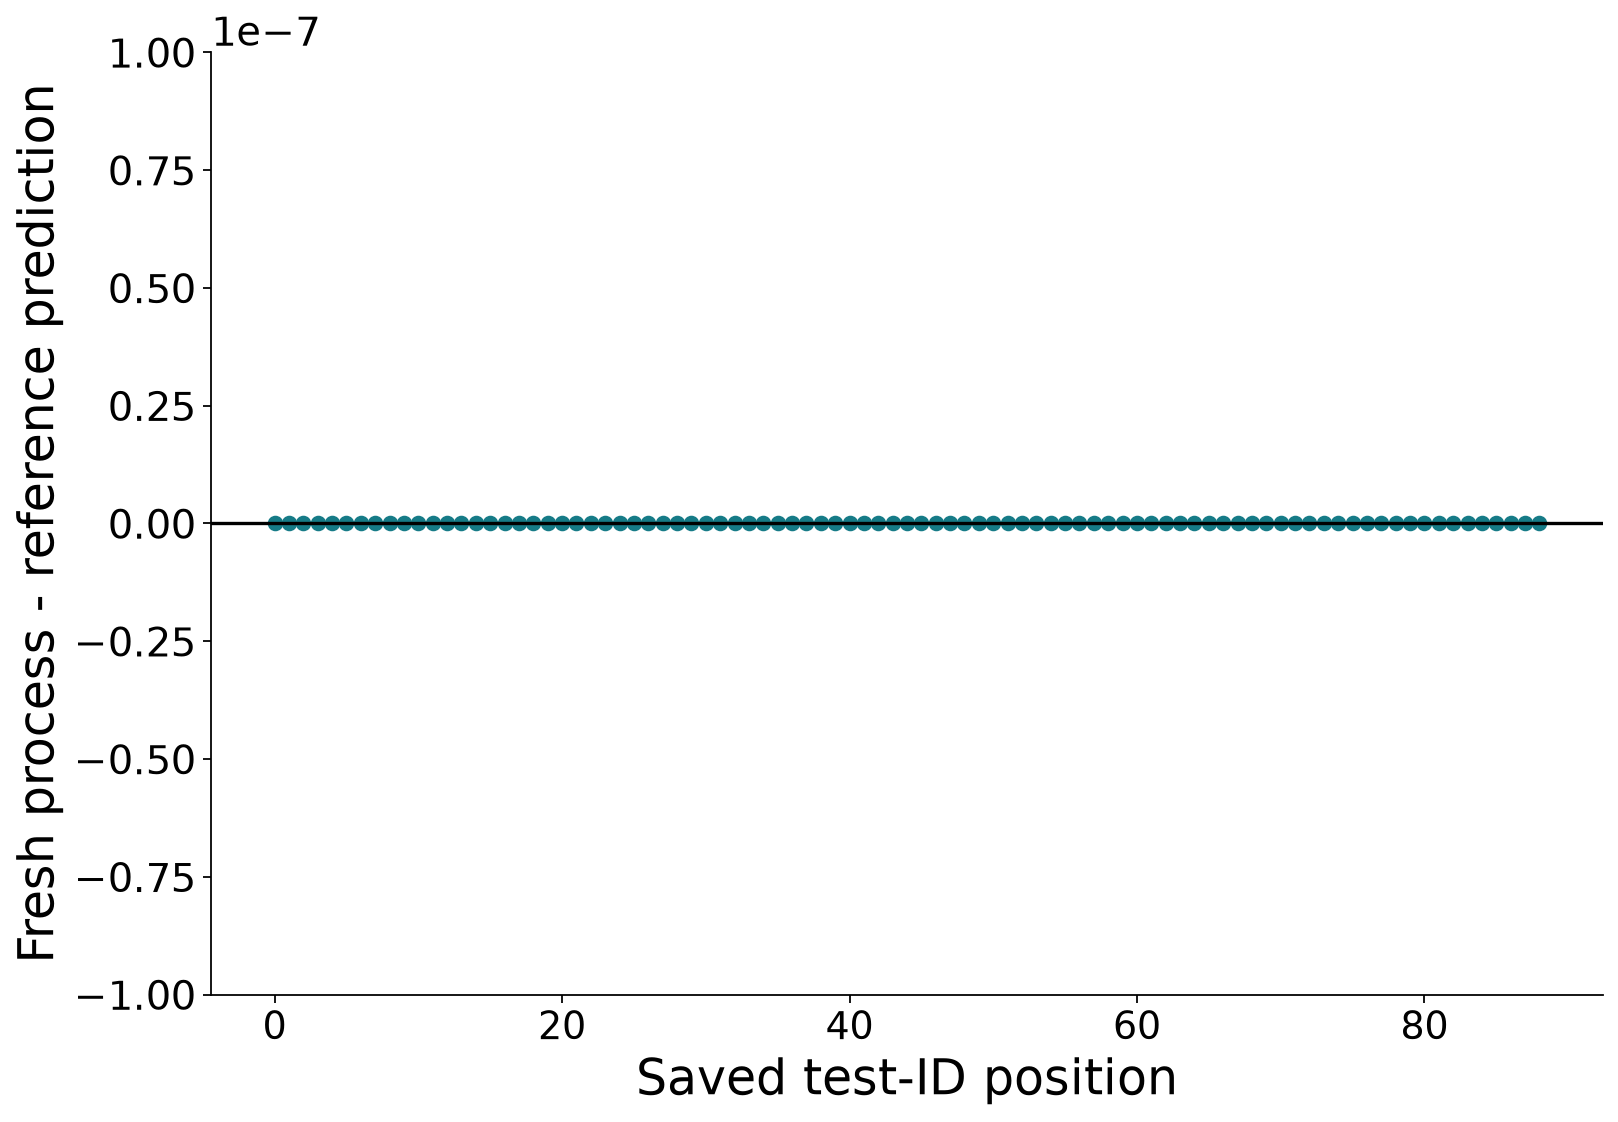
\includegraphics[width=.78\textwidth]{figures/week10/w10-replay-differences.png}\caption{Actual fresh-process prediction differences after exact ID alignment. The vertical scale is explicit. Replay difference and residual against observed target answer different questions.}\end{figure}

\section{Test deliberate failures on copies}
Corrupt only temporary copies of the data. The seven cases are a duplicate ID, non-finite value, reordered header, extra field, missing field, empty ID and invalid partition. Call the schema reader directly so no model is fitted during these contract tests. Catch the expected \texttt{ValueError} and record its message. An accepted malformed copy must trigger a failed assertion. Recheck the original data hash afterward.

\begin{figure}[htbp]\centering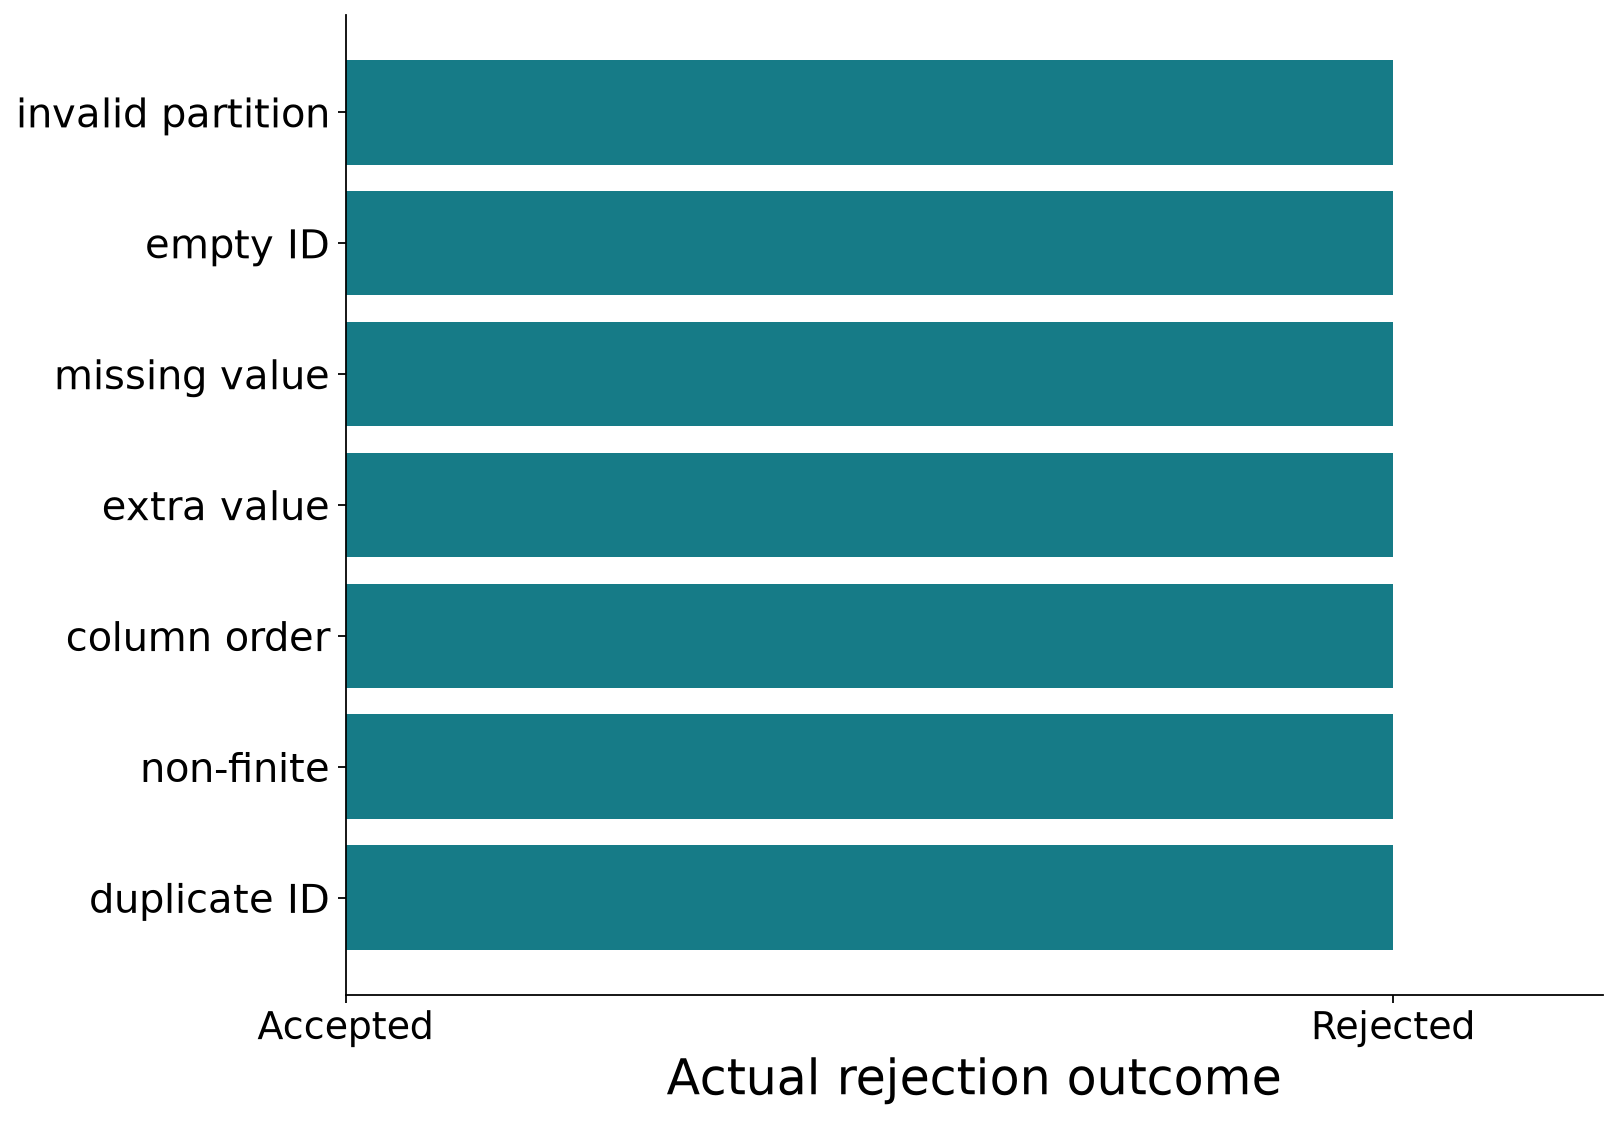
\includegraphics[width=.72\textwidth]{figures/week10/w10-contract-tests.png}\caption{Actual seven-case contract rejection test. These outcomes test an interface, not clinical safety or predictive accuracy.}\end{figure}


\section{Task 6 worked comparison: a legitimate row reorder}
A CSV's bytes encode row order; a model cohort is defined here by saved IDs. Reversing rows therefore changes the exact byte digest, while a complete ID-keyed record mapping can remain equal. The two claims need different checks:
\begin{enumerate}
\item Copy the frozen bundle and reverse only CSV data rows, retaining the header.
\item Compare the complete dictionary from source ID to every raw feature and target string. All keys and values must agree with the reference.
\item Record the reviewed transformation. Only then update the copied manifest's CSV digest; preserve the original manifest and file.
\item Run a new interpreter from a fresh working directory. The reader rebuilds training and test cohorts in the original saved ID sequence.
\item Compare the entire prediction vector. In the reference run the maximum difference is zero; record your own result.
\end{enumerate}
Updating a digest alone establishes no semantic equality. This exercise adds independent record and prediction checks. Optional A tests the opposite protocol: changed bytes with an unchanged manifest must be rejected. The selected model and its original evaluation are never reopened.

\subsection{Two numerical questions}
Model error compares predictions with observed targets: the selected model's test MAE remains approximately 48.326 response units in this reference run. Replay difference compares two computations of the same frozen prediction vector and is zero here. Neither quantity implies the other. An exact replay can faithfully reproduce a large error against an outcome.

\subsection{The receiver can test the extracted artifact}
After extracting the supplied ZIP and reviewing its source, run:
\begin{quote}\ttfamily\small
python handover/replay.py --root handover --out replay-result.json
\end{quote}
The JSON explicitly reports whether the saved reference comparison passed. No notebook variables are required. A missing required file, wrong reference ID order or incorrect numeric reference causes failure instead of a misleading success record. Instructor QA exercises these negative receiver cases as well as normal extraction.

\subsection{Practice timing and stopping conditions}
H1 uses Tasks1--2 (7 and8minutes); H2 uses Tasks3--5 (15,12 and18); H3 uses Tasks6--8 (15,12 and13), leaving20minutes for peer explanation, optional challenges and export. Read the Markdown purpose, instructions and stopping check before each cell. Save a prediction before executing; explain an actual output afterward. Missing variables after a runtime reset mean running from Setup again, not inserting a copied reference score.

\section{Eight core exercises and two optional challenges}
Each task requires a prediction before running, an actual observation, an explanation and a stopping check. Alternate driver and reviewer in pairs. Use H1 for Tasks 1--2, guided H2 for Tasks 3--5, and H3 for remaining work, review and export. These tasks share the 120 minutes of practice; they are not extra hours after the walkthrough.
\begin{enumerate}
\item \textbf{Row-order trap:} reverse a 20-ID toy dataset, reuse seeded positional indices, then recover the exact saved ID sequence. Explain why set equality alone is insufficient.
\item \textbf{Preprocessing scope:} assert the fitted scaler mean equals training means. Contrast all-row means descriptively without fitting a leaky competing model or claiming a particular score change.
\item \textbf{Selection rule:} recompute the validation-MAE winner and declared tie order. Never use final-test results to choose it.
\item \textbf{Contract failures:} reject all seven declared malformed cases on temporary copies. Confirm the original CSV unchanged.
\item \textbf{Fresh process:} copy the full bundle, execute its reviewed runner in another temporary working directory and inspect its standalone reference comparison. Check exact IDs and all89 predictions under the explicit tolerance.
\item \textbf{Reviewed row reorder:} reverse only the data rows of a temporary copied CSV. Verify equal ID-keyed records before updating that copy's CSV digest. Re-execute a fresh process, require the saved ID sequence and compare predictions. Preserve the reference bundle and selected candidate.
\item \textbf{Local explanation:} add $0.1$ training SD to one declared feature and verify the fitted-function prediction change. Record the candidate and exclude causal or clinical claims.
\item \textbf{Handover audit:} verify every payload digest and identify one actual failure row. Write claim, evidence, limitation and next evaluation so a partner can locate the supporting files.
\end{enumerate}
Optional A changes a copied CSV and confirms manifest rejection before training. Optional B explicitly restores reordered numeric columns by unique names and verifies exact recovery of the canonical matrix. Both preserve the reference package and neither is required for core completion.

\subsection{Student responses and evidence export}
The 19 core fields comprise eight predictions, eight explanations, controlled change, limitation and AI-use/checking disclosure (or ``none''). Student Exercise responses and published execution outputs start blank; the worked alternative contains example reasoning. Missing fields produce status \texttt{draft}; nonempty fields mean \texttt{ready for peer discussion}, not a correctness grade. Rerun only the final export after editing responses; initialization resets them. Every response cell is already supplied, so students do not need to insert new cells. Complete Tasks1--8 in order in one notebook, rather than performing a walkthrough and repeating the tasks afterward.

Download the single handover ZIP and save your edited notebook separately before the free runtime ends. The ZIP contains the frozen inner handover, actual plots and the outer response/evidence JSON. After code review, the extracted runner can be executed in a compatible environment using the explicit root and output paths shown in the notebook. No paid AI, GPU, API key or external dataset download is needed. AI may help explain code or suggest hypotheses, but it must not fabricate execution evidence or measured values.

\section{Instructor execution and limits}
On 27 October 2026 both notebooks were fully executed in fresh local CPU Jupyter kernels. Each invoked independent replay interpreters. All eight core tasks, both optional challenges, draft/completed export branches, all plot exports, numerical checks and ZIP integrity were checked. These are fresh local CPU kernels and separate interpreter checks; the Colab browser itself was not the execution environment. Actual versions are recorded in the evidence JSON; a local software check does not establish clinical, causal or external deployment validity.

\textbf{Reference CSV SHA-256:}\par\noindent{\small\texttt{a589d3035403d59869ec18c1007e379a396c9cc53b562cb979be676f2b85c4d4}}\par

\section{Summary and examination bridge}
Freeze identities, choices, transformations and environment. Reject malformed interfaces before fitting. Compare aligned prediction vectors in a new process, then state exactly what agreement supports. Keep predictive error, replay error, file integrity and scientific validity separate. For the written and oral midterm, be ready to explain one choice, one failure and one change that would invalidate the claim.

\section{Primary-source reading}
{\small\noindent\begin{tabular}{p{.46\linewidth}p{.46\linewidth}}
\href{https://scikit-learn.org/stable/modules/generated/sklearn.datasets.load_diabetes.html}{scikit-learn: raw dataset API} &
\href{https://scikit-learn.org/stable/common_pitfalls.html}{scikit-learn: preprocessing pitfalls}\\[4pt]
\href{https://scikit-learn.org/stable/model_persistence.html}{scikit-learn: persistence and security} &
\href{https://numpy.org/doc/stable/reference/random/compatibility.html}{NumPy: random-stream compatibility}
\end{tabular}}

